\section{Progettazione logica}

\subsection{Ristrutturazione dello schema}

\subsubsection{Analisi delle ridondanze}
\begin{enumerate}

\item Inserimento di un attributo \textbf{Totale} in \underline{Acquisto}:

Si tratta di un attributo derivato calcolabile dalla somma dei singoli prezzi dei \textbf{componenti} che formano l'acquisto. \\
Si considerano le seguenti due operazioni che coinvolgono la base di dati, per analizzare la sua efficienza in presenza o meno dell'attributo ridondante:\\

\begin{itemize}
\item \underline{Operazione 1)} Registrazione di un nuovo acquisto nella base di dati.
\item \underline{Operazione 2)} Lettura giornaliera del fatturato, ossia del totale del denaro riscattato in seguito alle vendite giornaliere.\\
\end{itemize}

Si suppone che in media vengano registrati \textbf{10 acquisti di componenti}, ciascuno dei quali sia formato da un numero significativo di componenti, adatto ad assemblare correttamente un pc. Verranno considerati quindi \textbf{8 componenti} per ogni acquisto.\\

\begin{itemize}

\item In caso di \textbf{Presenza dell'attributo ridondante}:\\

Operazione 1) 
\begin{tabular}{|c|c|c|c|}
\hline
\rowcolor{LightCyan}
\centered{\textbf{Concetto}}&\centered{\textbf{Costrutto}}&\centered{\textbf{Accessi}}&\centered{\textbf{Tipo}}\\
\hline
\centered{Acquisto} & \centered{Entita'} & \centered{1} & \centered{S}\\
\hline
\centered{Acquisto\_Componenti} & \centered{Entita'} & \centered{1} & \centered{S}\\
\hline
\centered{Composizione} & \centered{Relazione} & \centered{8} & \centered{S}\\
\hline
\centered{Componente} & \centered{Entita'} & \centered{8} & \centered{L}\\
\hline
\end{tabular}\\

Si attribuisce alle operazioni in scrittura un peso doppio rispetto a quelle in lettura, quindi un singolo acquisto per essere registrato porta ad un costo complessivo di (1 * 2) + (1 * 2) + (8 * 2) + 8 = \textbf{28 accessi}. Questa operazio abbiamo definito essere eseguita in media circa 10 volte al giorno, quindi porta ad un totale di \textbf{280 accessi} giornalieri.\\



Operazione 2) 
\begin{tabular}{|c|c|c|c|}
\hline
\rowcolor{LightCyan}
\centered{\textbf{Concetto}}&\centered{\textbf{Costrutto}}&\centered{\textbf{Accessi}}&\centered{\textbf{Tipo}}\\
\hline
\centered{Acquisto\_Componenti} & \centered{Entita'} & \centered{1} & \centered{L}\\
\hline
\centered{Acquisto} & \centered{Entita'} & \centered{1} & \centered{L}\\
\hline
\end{tabular}\\

Il costo totale dell'operazione 2 e' dunque di (1 + 1) * 10 =\textbf{20 accessi}.\\


\item In caso di \textbf{Assenza dell' attributo ridondante}:\\

Operazione 1) 
\begin{tabular}{|c|c|c|c|}
\hline
\rowcolor{LightCyan}
\centered{\textbf{Concetto}}&\centered{\textbf{Costrutto}}&\centered{\textbf{Accessi}}&\centered{\textbf{Tipo}}\\
\hline
\centered{Acquisto} & \centered{Entita'} & \centered{1} & \centered{S}\\
\hline
\centered{Acquisto\_Componenti} & \centered{Entita'} & \centered{1} & \centered{S}\\
\hline
\centered{Composizione} & \centered{Relazione} & \centered{8} & \centered{S}\\
\hline
\centered{Componente} & \centered{Entita'} & \centered{8} & \centered{L}\\
\hline
\end{tabular}\\

Si noti che in assenza dell'attributo ridondante, l'operazione 1 richiede esattamente gli stessi accessi che tenevano conto dell'attributo. Questo perche' l'inserimento di un acquisto e' indipendente da tale attributo.\\


Operazione 2) 
\begin{tabular}{|c|c|c|c|}
\hline
\rowcolor{LightCyan}
\centered{\textbf{Concetto}}&\centered{\textbf{Costrutto}}&\centered{\textbf{Accessi}}&\centered{\textbf{Tipo}}\\
\hline
\centered{Acquisto\_componenti} & \centered{Entita'} & \centered{1} & \centered{L}\\
\hline
\centered{Composizione} & \centered{Relazione} & \centered{8} & \centered{L}\\
\hline
\centered{Componente} & \centered{Entita'} & \centered{8} & \centered{L}\\
\hline
\end{tabular}\\

Si denota dunque che con un totale di (1 + 8 + 8) * 10= \textbf{170 accessi}, l'assenza di un attributo ridondante per il totale del prezzo della vendita porta a dei rallentamenti nell'interrogazione del database in caso di operazioni attuate quotidianamente.\\
In seguito a tale analisi si decide di mantenere la presenza dell'attributo ridondante \textbf{Totale} nell'entita' \underline{Acquisto}.\\
\end{itemize}


\item Inserimento di un atttributo \textbf{Prezzo} in \underline{PC}:\\

Si tratta di un attributo derivato calcolabile dalla somma dei singoli prezzi dei \textbf{componenti} che compongono la configurazione del PC e il costo relativo all'assemblaggio dei componenti. Quest'ultimo si riferisce al costo aggiuntivo che il negozio deve pagare al momento dell'acquisto di un PC pre-assemblato.
In genere tale costo aggiuntivo risulta essere il 25\% del prezzo totale dei componenti presenti nel pc.\\
Si considerino dunque le seguenti operazioni:\\

\begin{itemize}
\item \underline{Operazione 1)} Registrazione nel database di un nuovo PC pre-assemblato.
\item \underline{Operazione 2)} Calcolo del fatturato delle vendite relative ai PC pre-assemblati.\\
\end{itemize}

Anche in questo caso si suppone che i componenti che formano un pc siano in media 8. La frequenza media stimata per l'esecuzione della prima operazione e' di 3 volte al giorno. Si presume dunque che vengano registrate tante vendite quante sono le registrazioni di nuovi PC pre-assemblati.\\

\begin{itemize}
\item In caso di \textbf{Presenza dell'attributo ridondante}:\\

Operazione 1)
\begin{tabular}{|c|c|c|c|}
\hline
\rowcolor{LightCyan}
\centered{\textbf{Concetto}}&\centered{\textbf{Costrutto}}&\centered{\textbf{Accessi}}&\centered{\textbf{Tipo}}\\
\hline
\centered{PC} & \centered{Entita'} & \centered{1} & \centered{S}\\
\hline
\centered{Configurazione} & \centered{Relazione} & \centered{8} & \centered{S}\\
\hline
\centered{Componente} & \centered{Entita'} & \centered{8} & \centered{L}\\
\hline
\end{tabular}\\

Dunque ogni registrazione di un pc porta ad un numero pari a (1 * 2) + (8 * 2) + 8 = \textbf{26 accessi}, che considerando la frequenza con cui tale operazione viene eseguita, porta ad un totale di 26 * 5 = \textbf{130 accessi} giornalieri.\\

Operazione 2) 
\begin{tabular}{|c|c|c|c|}
\hline
\rowcolor{LightCyan}
\centered{\textbf{Concetto}}&\centered{\textbf{Costrutto}}&\centered{\textbf{Accessi}}&\centered{\textbf{Tipo}}\\
\hline
\centered{Acquisto\_PC} & \centered{Entita'} & \centered{1} & \centered{L}\\
\hline
\centered{Composizione} & \centered{Relazione} & \centered{1} & \centered{L}\\
\hline
\centered{PC} & \centered{Entita'} & \centered{1} & \centered{L}\\
\hline
\end{tabular}\\ 

Quest'operazione porta dunque ad un costo di (1 + 1 + 1) * 5 = \textbf{15 accessi} giornalieri.\\

\item In caso di \textbf{Assenza dell' attributo ridondante}:\\

Per l'operazione 1) analogamente a quanto visto in precedenza nell'analisi di ridondanza per l'inserimento di un attributo totale ad acquisto, il numero di accessi non dipende dalla presenza dell'attributo ridondante e non aggiunge quindi complessita' all'operazione. Il numero di accessi risulta dunque essere anche in questo caso pari a \textbf{130 accessi}.\\

Operazione 2)
\begin{tabular}{|c|c|c|c|}
\hline
\rowcolor{LightCyan}
\centered{\textbf{Concetto}}&\centered{\textbf{Costrutto}}&\centered{\textbf{Accessi}}&\centered{\textbf{Tipo}}\\
\hline
\centered{Acquisto\_PC} & \centered{Entita'} & \centered{1} & \centered{L}\\
\hline
\centered{Composizione} & \centered{Relazione} & \centered{1} & \centered{L}\\
\hline
\centered{PC} & \centered{Entita'} & \centered{1} & \centered{L}\\
\hline
\centered{Configurazione} & \centered{Relazione} & \centered{8} & \centered{L}\\
\hline
\centered{Componente} & \centered{Entita'} & \centered{8} & \centered{L}\\
\hline 
\end{tabular}\\ 

Si denota dunque come, anche in questo caso, in assenza di un attributo ridondante il numero di accessi giornalieri sia di gran lunga maggiore rispetto al caso in cui vi sia l'attributo ridondante. Per l'operazione infatti sono necessari (1 + 1 + 1 + 8 + 8) * 5 = \textbf{95 accessi} rispetto ai 15 calcolati in precedenza.
Si manterra' dunque la presenza di un attibuto \textbf{Prezzo} nell'entita' \underline{PC}.\\
Questo campo inoltre, per rappresentare il totale di un acquisto, corrispondera' al campo totale nell'entita' acquisti, dove l'acquisto si riferisce a PC pre-assemblati.
\end{itemize}


\end{enumerate}


\subsubsection{Politiche di ristrutturazione dello schema}

Lo schema, a seguito dell' analisi delle ridondanze e di alcune considerazioni verra' ristrutturato tenendo conto dei seguenti punti fondamentali:
\begin{itemize}
\item Aggiunta di attributi ridondanti a seguito delle analisi riportate nella precedente sezione.
\item Eliminazione della generalizzazione riguardante l' entita' padre \underline{Dipendente} attraverso l'\textbf{accorpamento} delle entita' figlie al padre e l' aggiunta di un relativo campo \textbf{'Mansione'}.
\item Eliminazione della generalizzazione riguardante l' entita' \underline{Acquisto}, mediante la \textbf{creazione di relazioni} tra Acquisto e le sue entita' figlie Acquisto\_Componenti e Acquisto\_Preassemblati.
\item Eliminazione della sottogeneralizzazione di \underline{Acquisto\_Componenti} mediante l' \textbf{accorpamento} delle entita' figlie Conluso e Non concluso al padre. Viene aggiunto un campo Concluso di tipo bool per rappresentare la differenza tra i tipi di Acquisto\_Componenti.\\
\end{itemize}

In seguito riportiamo dunque lo schema ristrutturato:\\
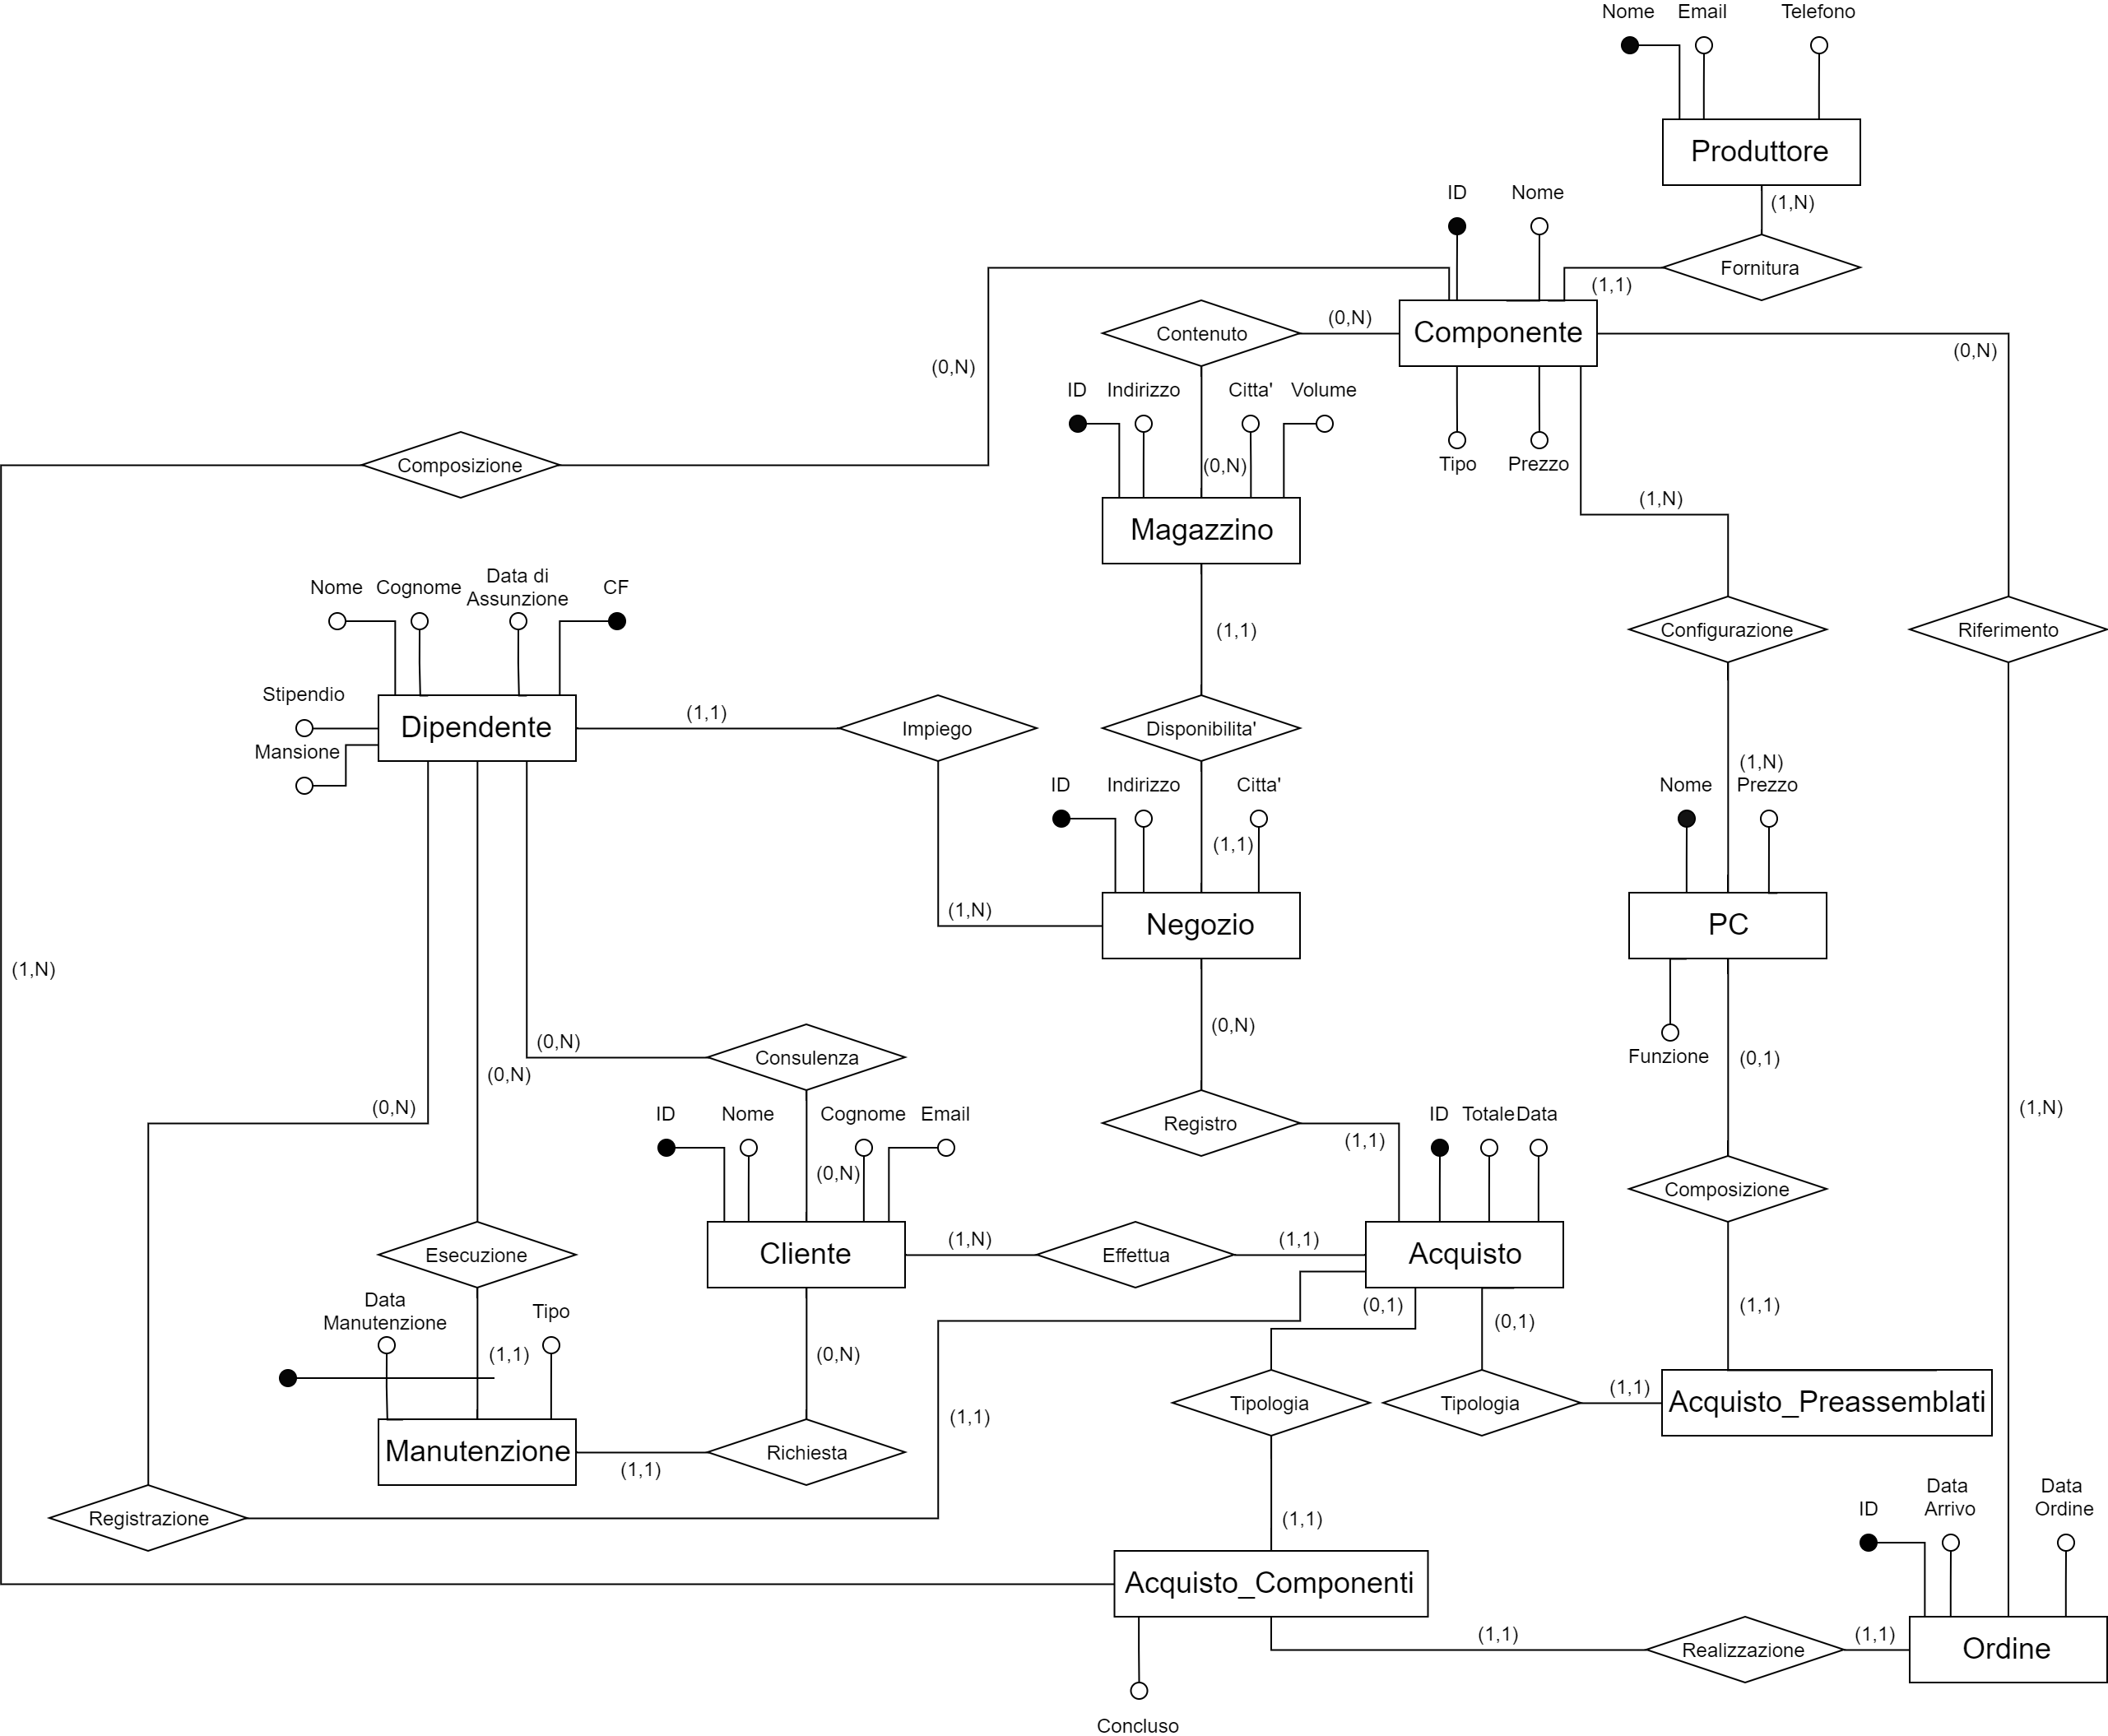
\includegraphics[scale=0.18]{ER-Ristrutturato}